\chapter{التنظيم الوظيفي عند الثدييات}\label{ch:b1:mammal-organization}

افتح أرنبًا على لوح التشريح فيكون الانطباع الأول انطباع نظام. صفيحة
عضلية، هي \omterm{def:b1:mammal-organization:bodyplan}{الحجاب الحاجز}، تقسم الجذع إلى صدر يحوي القلب والرئتين،
وبطن يحوي كل ما عداهما: كبد بحجم القبضة، ومعدة، وأربعة أمتار من
المعي تنتهي بأعور في حجم المعدة، وكليتان ملتصقتان بالجدار الخلفي.
لكل \omterm{def:b1:mammal-organization:organ}{عضو} موضع، وإمداد دموي، وعمل؛ ولا يعمل أي منها وحده. يصف هذا
الفصل كيف يُبنى الثديي كلًا يعمل: مخططه التنظيمي، والأجهزة التي
تُجمع فيها أعضاؤه، والحجيرات السائلة التي تعيش فيها خلاياه، وسطوح
التبادل التي يلاقي بها الخارج، \omterm{prop:b1:mammal-organization:heatbudget}{والميزانية الحرارية} التي تبقيه عند
\qty{39}{\celsius} في حقل من حقول يناير.

\section{المخطط التنظيمي عند الثدييات}

\begin{definition}[المخطط التنظيمي]\label{def:b1:mammal-organization:bodyplan}
\emph{المخطط التنظيمي}\index{مخطط تنظيمي} لحيوان هو ترتيب محاوره
وأجوافه وأعضائه المشترك بين كل أفراد مجموعته. والمخطط التنظيمي عند
الثدييات هو مخطط الفقاريات: تناظر جانبي، ونهاية رأسية تحمل الدماغ
\omterm{def:b1:mammal-organization:organ}{وأعضاء} الحس الرئيسة (\emph{التمركز الرأسي}\index{التمركز الرأسي})،
ومحور ظهري من الفقرات يحيط بالنخاع الشوكي، وأربعة أطراف، وجوف بطني
--- هو \emph{الجوف العام}\index{الجوف العام} --- يحوي الأحشاء. أما ما
هو خاص بالثدييات فهو: أن \emph{الحجاب الحاجز}\index{الحجاب الحاجز}
العضلي يقسم الجوف العام إلى جوف صدري (القلب، والرئتان) وجوف بطني
(\omterm{def:b1:mammal-organization:organ}{أعضاء} الهضم، والكليتان، والمناسل)؛ وأن الجسم مغطى بالشعر؛ وأن
الصغار تُغذَّى باللبن؛ وأن درجة الحرارة منظَّمة.
\end{definition}

\begin{omfigure}
\begin{tikzpicture}
  \node[anchor=south west, inner sep=0] (img) at (0,0)
    {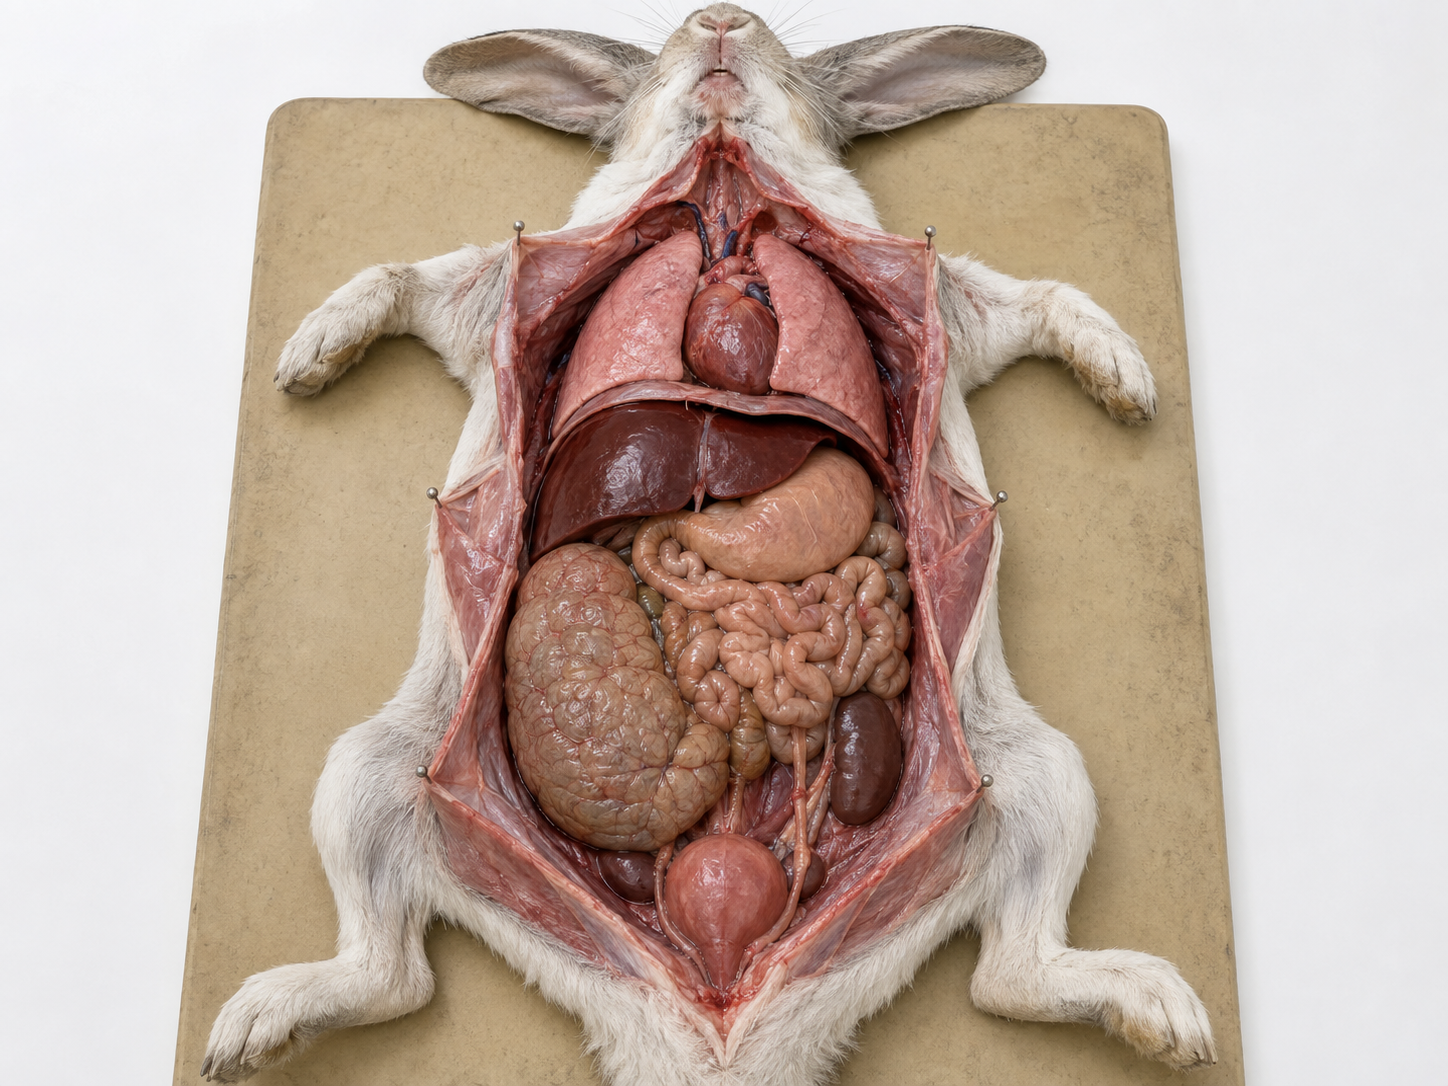
\includegraphics[width=0.6\linewidth]{images/book3/ai/fig-rabbit-dissection.png}};
  \begin{scope}[x={(img.south east)}, y={(img.north west)},
      every node/.style={font=\small}]
    \draw[omDef, thick] (0.44,0.72) -- (-0.02,0.90) node[left] {رئتان};
    \draw[omDef, thick] (0.50,0.68) -- (1.02,0.88) node[right] {قلب};
    \draw[omDef, thick] (0.53,0.61) -- (1.02,0.70) node[right] {حجاب حاجز};
    \draw[omDef, thick] (0.44,0.55) -- (-0.02,0.62) node[left] {كبد};
    \draw[omDef, thick] (0.56,0.52) -- (1.02,0.54) node[right] {معدة};
    \draw[omDef, thick] (0.52,0.42) -- (1.02,0.40) node[right] {معي دقيق};
    \draw[omDef, thick] (0.42,0.36) -- (-0.02,0.36) node[left] {أعور};
    \draw[omDef, thick] (0.60,0.30) -- (1.02,0.24) node[right] {كلية};
    \draw[omDef, thick] (0.51,0.17) -- (-0.02,0.10) node[left] {مثانة};
  \end{scope}
\end{tikzpicture}

{\small أرنب مفتوح من الجهة البطنية. \omterm{def:b1:mammal-organization:bodyplan}{الحجاب الحاجز} يفصل الجوف الصدري
(الرئتان، والقلب) عن الجوف البطني (الكبد، والمعدة، والمعي، والأعور،
والكليتان، والمثانة). ولكل \omterm{def:b1:mammal-organization:organ}{عضو} موضع ثابت، ملفوف في غشاء، تمده أوعيته
الخاصة.}
\end{omfigure}

\begin{definition}[العضو، الجهاز]\label{def:b1:mammal-organization:organ}
\emph{العضو}\index{عضو} بنية مكونة من عدة أنسجة
(\cref{ch:b1:body-plans-tissues}) مرتبة لأداء وظيفة محددة: فالقلب
يضخ، والرئة تبادل الغازات، والكلية ترشح. و\emph{الجهاز}\index{جهاز}
مجموعة أعضاء تتعاون في وظيفة عامة واحدة: فالجهاز الهضمي يمتد من الفم
إلى الشرج ويتصل به الكبد والبنكرياس؛ والجهاز الدوراني هو القلب
والأوعية؛ والجهاز الإطراحي هو الكليتان والمسالك البولية.
\end{definition}

\section{الأجهزة والوظائف التي تخدمها}

\begin{proposition}[ثلاث مجموعات من الوظائف]\label{prop:b1:mammal-organization:functions}
تخدم أجهزة الثديي ثلاث مجموعات من الوظائف:
\begin{itemize}
  \item \emph{التغذية}\index{وظيفة التغذية}: أخذ المادة والطاقة
        وتوزيعهما وطرح الفضلات --- \omterm{def:b1:mammal-organization:organ}{الجهاز} الهضمي، والتنفسي،
        والدوراني، والإطراحي؛
  \item \emph{العلاقة}\index{وظيفة العلاقة}: الإحساس \omterm{def:b1:organism-environment:organism}{بالمحيط} والفعل
        فيه --- \omterm{def:b1:mammal-organization:organ}{أعضاء} الحس، \omterm{def:b1:mammal-organization:organ}{والجهاز} العصبي، والغدد الصماء، والهيكل،
        والعضلات؛
  \item \emph{التكاثر}\index{وظيفة التكاثر}: إنتاج الذرية ---
        المناسل، والسبيل التناسلي، والغدد اللبنية عند الثدييات.
\end{itemize}
ولا يعمل \omterm{def:b1:mammal-organization:organ}{جهاز} وحده: فكل \omterm{def:b1:mammal-organization:organ}{عضو} يعتمد على الدم في إمداده، وعلى الجهازين
العصبي والصماوي في تنسيقه، وعلى الهيكل والجلد في حمايته.
\end{proposition}

\begin{omfigure}
\begin{tikzpicture}[font=\footnotesize, >=Stealth, line cap=round,
  sys/.style={draw, thick, rounded corners=3pt, minimum height=7mm, minimum width=24mm, align=center, fill=white},
  lab/.style={font=\scriptsize, above},
  grp/.style={font=\small\bfseries, anchor=west}]
  \node[grp, omProp] at (0,4.6) {التغذية};
  \node[sys, fill=omProp!12] (dig) at (1.3,3.8) {هضمي};
  \node[sys, fill=omProp!12] (res) at (1.3,2.9) {تنفسي};
  \node[sys, fill=omProp!12] (exc) at (1.3,2.0) {إطراحي};
  \node[grp, omExo] at (0,1.1) {التكاثر};
  \node[sys, fill=omExo!12] (gen) at (1.3,0.3) {تناسلي};
  \node[sys, fill=omThm!12, minimum height=30mm] (cir) at (5.9,2.6) {دوراني\\ (دم، لمف)};
  \node[grp, omDef] at (8.6,4.6) {العلاقة};
  \node[sys, fill=omDef!12, minimum width=30mm] (ner) at (10.3,3.8) {عصبي، حواس};
  \node[sys, fill=omDef!12, minimum width=30mm] (end) at (10.3,2.9) {صماوي};
  \node[sys, fill=omDef!12, minimum width=30mm] (mus) at (10.3,2.0) {هيكل، عضلات};
  \node[sys, fill=omDef!12, minimum width=30mm] (ski) at (10.3,1.1) {جلد};
  \draw[<->, thick] (dig.east) -- (cir.west |- dig.east) node[lab, midway] {مغذيات};
  \draw[<->, thick] (res.east) -- (cir.west |- res.east) node[lab, midway] {$\mathrm{O_2}$, $\mathrm{CO_2}$};
  \draw[<->, thick] (exc.east) -- (cir.west |- exc.east) node[lab, midway] {فضلات};
  \draw[<->, thick] (gen.east) -- ++(1.6,0) |- (cir.south west);
  \draw[<->, thick] (cir.east |- ner.west) -- (ner.west);
  \draw[<->, thick] (cir.east |- end.west) -- (end.west) node[lab, midway] {هرمونات};
  \draw[<->, thick] (cir.east |- mus.west) -- (mus.west);
  \draw[<->, thick] (cir.south east) -| ++(0.5,0) |- (ski.west);
\end{tikzpicture}

{\small أجهزة الثديي مجموعة بحسب الوظيفة. الدوران هو المحور: فكل
\omterm{def:b1:mammal-organization:organ}{جهاز} يتبادل مع الدم، والدم يحمل ما يأخذه \omterm{def:b1:mammal-organization:organ}{جهاز} إلى كل \omterm{def:b1:mammal-organization:organ}{جهاز} آخر.}
\end{omfigure}

\begin{example}[لقمة عشب]\label{ex:b1:mammal-organization:mouthful}
عشب الأرنب تقطعه القواطع وتطحنه الأضراس (الهيكل والعضلات)، ويُذاق
ويُشم (الحواس)، ويُبلع ويُهضم في المعدة والمعي الدقيق؛ وتعبر سكرياته
وحموضه الأمينية جدار المعي إلى الدم فتبلغ الكبد، الذي يخزنها أو
يطلقها تحت تحكم هرموني (\omterm{def:b1:mammal-organization:organ}{الجهاز} الصماوي)؛ وتُخمَّر سليولوزه ببكتيريا
الأعور؛ ويأتي الأكسجين اللازم لحرق السكريات عبر الرئتين، ويخرج ثاني
أكسيد الكربون من الطريق نفسه، وتخرج البولة الآتية من الحموض الأمينية
عبر الكليتين، وتخرج حرارة العملية كلها عبر الجلد. سبعة أجهزة للقمة
واحدة.
\end{example}

\section{حجيرات الجسم}

\begin{definition}[الحجيرات السائلة]\label{def:b1:mammal-organization:compartments}
يشكل الماء نحو \qty{60}{\%} من كتلة الثديي. ثلثاه \emph{سائل داخل
خلوي}\index{السائل داخل الخلوي}، في داخل الخلايا؛ وثلثه \emph{سائل
خارج خلوي}\index{السائل خارج الخلوي}، وهو \omterm{def:b1:organism-environment:milieu}{الوسط الداخلي} في
\cref{ch:b1:organism-environment}، وينقسم بدوره إلى \emph{السائل
الخلالي}\index{السائل الخلالي} الذي يغمر الخلايا (ثلاثة أرباعه)
و\emph{بلازما الدم}\index{بلازما} داخل الأوعية (الربع).
و\emph{اللمف}\index{لمف} سائل خلالي تجمعه الأوعية اللمفية وتعيده إلى
الدم. وللسائلين خارج الخلويين تركيب واحد تقريبًا --- تختلف البلازما
ببروتيناتها التي لا تعبر جدار الشعرية --- ويختلفان كلاهما اختلافًا
حادًا عن السائل داخل الخلوي.
\end{definition}

\begin{omfigure}
\begin{tikzpicture}[font=\small, line cap=round]
  \draw[thick, fill=gray!8, rounded corners=6pt] (0,0) rectangle (11.6,4.6);
  \node[anchor=north west, font=\small\bfseries] at (0.15,4.55) {مجموع ماء الجسم: \qty{42}{L} (\qty{60}{\%} من \qty{70}{kg})};
  \draw[thick, fill=omDef!14, rounded corners=5pt] (0.3,0.3) rectangle (6.4,3.8);
  \node[anchor=north west, align=left] at (0.4,3.7) {\textbf{السائل داخل الخلوي}: \qty{28}{L}\\ $\mathrm{K^+}$ مرتفع (\qty{140}{mmol/L})،\\ فوسفات، بروتينات؛\\ $\mathrm{Na^+}$ منخفض (\qty{10}{mmol/L})};
  \draw[thick, fill=omProp!14, rounded corners=5pt] (6.7,0.3) rectangle (11.3,3.8);
  \node[anchor=north west, align=left] at (6.8,3.7) {\textbf{السائل خارج الخلوي}: \qty{14}{L}\\ $\mathrm{Na^+}$ مرتفع (\qty{140}{mmol/L})،\\ $\mathrm{Cl^-}$، $\mathrm{HCO_3^-}$};
  \draw[thick, fill=omProp!30, rounded corners=4pt] (6.9,0.45) rectangle (9.2,1.55);
  \node[align=center, font=\footnotesize] at (8.05,1.0) {خلالي\\ \qty{11}{L}};
  \draw[thick, fill=omThm!30, rounded corners=4pt] (9.4,0.45) rectangle (11.1,1.55);
  \node[align=center, font=\footnotesize] at (10.25,1.0) {بلازما\\ \qty{3}{L}};
\end{tikzpicture}

{\small الحجيرات السائلة عند إنسان كتلته \qty{70}{kg}. ثلثا الماء
داخل الخلايا؛ والثلث خارج الخلوي، الموزع بين \omterm{def:b1:mammal-organization:compartments}{السائل الخلالي}
والبلازما، هو \omterm{def:b1:organism-environment:milieu}{الوسط الداخلي}. والصوديوم مسيطر في الخارج، والبوتاسيوم
في الداخل --- وهو فرق تنفق كل خلية طاقة لصونه
(\cref{ch:b1:membranes-transport}).}
\end{omfigure}

\begin{method}[قياس حجيرة بالتمديد]\label{met:b1:mammal-organization:dilution}
\begin{enumerate}
  \item اختر واسمًا ينتشر في الحجيرة ولا ينتشر في غيرها: صباغًا
        يرتبط ببروتينات البلازما (أزرق إيفانز) للبلازما؛ والإينولين،
        وهو سكر يغادر الأوعية ولا يدخل الخلايا، \omterm{def:b1:mammal-organization:compartments}{للسائل خارج الخلوي}؛
        والماء الثقيل لمجموع ماء الجسم.
  \item احقن كمية معلومة $m$ وانتظر الامتزاج (دقائق للبلازما، وساعات
        لمجموع الماء).
  \item قِس التركيز $c$ في عينة من البلازما، مصححًا كل فقد (بول،
        استقلاب) خلال الانتظار.
  \item الحجم هو $V = m/c$. والحجم داخل الخلوي هو مجموع الماء ناقص
        خارج الخلوي؛ والحجم الخلالي هو خارج الخلوي ناقص البلازما.
        وحجم الدم هو حجم البلازما مقسومًا على كسر البلازما من الدم
        ($1 - $ الهيماتوكريت).
\end{enumerate}
\end{method}

\begin{example}[حجم بلازما]\label{ex:b1:mammal-organization:evansblue}
\qty{50}{mg} من أزرق إيفانز محقونة في رجل كتلته \qty{70}{kg} تعطي،
بعد عشر دقائق، تركيزًا في البلازما قدره \qty{16.7}{mg/L}:
$V = 50/16.7 = \qty{3.0}{L}$ من البلازما. وبهيماتوكريت
\qty{45}{\%} يكون حجم الدم $3.0/0.55 = \qty{5.5}{L}$ --- أي
\qty{8}{\%} من كتلة الجسم، وهي نسبة تصدق من الفأر إلى الحوت.
\end{example}

\section{سطوح التبادل والدوران}

\begin{proposition}[كل سطح تبادل مقترن بالدم]\label{prop:b1:mammal-organization:surfaces}
يتبادل الثديي مع الخارج عبر أربعة سطوح، كل منها مطوي داخل الجسم
وكل منها مروي بشبكة شعرية كثيفة: مخاطية المعي (\qty{30}{m^2} عند
الإنسان) للمغذيات والماء، والسطح السنخي في الرئتين (\qty{100}{m^2})
للأكسجين وثاني أكسيد الكربون، والسطح الراشح في الكليتين (مليون
كبيبة، ترشح \qty{180}{L} من البلازما في اليوم) للفضلات ولتنظيم \omterm{def:b1:organism-environment:milieu}{الوسط
الداخلي}، والجلد (\qty{2}{m^2}) للحرارة ولقليل من الماء. والدوران
يربط بينها: فالدم الخارج من سطح يبلغ السطح التالي في دقيقة، حتى إن
ما يدخل عبر المعي يُؤكسد بأكسجين آت من الرئة وتخرج فضلته عبر
الكلية.
\end{proposition}

\begin{omfigure}
\begin{tikzpicture}[font=\small, >=Stealth, line cap=round,
  org/.style={draw, thick, rounded corners=4pt, minimum height=8mm, minimum width=22mm, align=center, fill=white}]
  \node[org, fill=omDef!12] (lung) at (0,3.2) {رئتان\\ \qty{100}{m^2}};
  \node[org, fill=omThm!15, minimum width=26mm, minimum height=12mm] (heart) at (0,0) {قلب\\ أيمن $\mid$ أيسر};
  \node[org, fill=omProp!12] (gut) at (5.2,1.6) {معي\\ \qty{30}{m^2}};
  \node[org, fill=omProp!12] (liver) at (5.2,0.0) {كبد};
  \node[org, fill=omProp!12] (kid) at (5.2,-1.6) {كليتان\\ \qty{180}{L/d}};
  \node[org, fill=omExo!12] (mus) at (5.2,3.2) {عضلات، جلد،\\ دماغ، وغيرها};
  % pulmonary loop
  \draw[->, very thick, omDef] (heart.north west) ++(-0.2,0) |- (lung.west) node[pos=0.25, left, font=\footnotesize, align=right] {الدوران\\ الرئوي};
  \draw[->, very thick, omThm] (lung.east) -| ($(heart.north east)+(0.2,0)$);
  % systemic loop: left heart -> organs (parallel) -> right heart
  \draw[very thick, omThm] (heart.east) -- ++(1.2,0) coordinate (a);
  \draw[->, very thick, omThm] (a) |- (mus.west);
  \draw[->, very thick, omThm] (a) |- (gut.west);
  \draw[->, very thick, omThm] (a) |- (kid.west);
  \draw[->, very thick, omThm] (a) -- (liver.west);
  \draw[->, very thick, omDef] (gut.south) -- (liver.north) node[midway, right, font=\footnotesize] {الوريد البابي};
  \coordinate (b) at (8.0,0.8);
  \draw[very thick, omDef] (mus.east) -| (b);
  \draw[very thick, omDef] (liver.east) -| (b);
  \draw[very thick, omDef] (kid.east) -| (b);
  \draw[->, very thick, omDef] (b) |- ++(0,-3.2) -| (heart.south) node[pos=0.25, below, font=\footnotesize] {الدوران العام: الأوردة};
\end{tikzpicture}

{\small الدوران المضاعف عند الثدييات. القلب الأيمن يرسل الدم الفقير
بالأكسجين (أزرق) عبر الرئتين؛ والقلب الأيسر يرسل الدم المؤكسج (أحمر)
عبر \omterm{def:b1:mammal-organization:organ}{الأعضاء} المرتبة على التوازي، فينال كل منها دمًا شريانيًا طازجًا.
والدم الآتي من المعي يمر عبر الكبد قبل عودته إلى القلب.}
\end{omfigure}

\begin{omfigure}
\begin{tikzpicture}
\begin{axis}[
  xbar, bar width=8pt,
  width=0.82\linewidth, height=6.2cm,
  axis x line=bottom, axis y line=left,
  xmin=0, xmax=1.8, xlabel={جريان الدم في الراحة (\unit{L/min})},
  xlabel style={font=\small, at={(axis description cs:0.5,-0.13)}, anchor=north},
  symbolic y coords={عضلة القلب, الجلد, الدماغ, العضلات الهيكلية, الكليتان, الكبد والمعي},
  ytick=data, tick label style={font=\small},
  enlarge y limits=0.12, xtick={0,0.5,1.0,1.5},
  nodes near coords, nodes near coords style={font=\scriptsize, anchor=west},
]
\addplot[fill=omThm!45, draw=omThm] coordinates
  {(0.25,عضلة القلب) (0.4,الجلد) (0.75,الدماغ) (1.0,العضلات الهيكلية) (1.1,الكليتان) (1.35,الكبد والمعي)};
\end{axis}
\end{tikzpicture}

{\small كيف يُقتسم صبيب قلبي بشري قدره \qty{5}{L/min} في الراحة بين
\omterm{def:b1:mammal-organization:organ}{الأعضاء}. الكليتان، وهما \qty{0.5}{\%} من كتلة الجسم، تأخذان خمس
الدم --- وهو ثمن ترشيح البلازما كلها ستين مرة في اليوم. وفي الجهد
يرتفع نصيب العضلات عشرة أضعاف ويهبط نصيب المعي.}
\end{omfigure}

\begin{example}[زمن الدوران]\label{ex:b1:mammal-organization:circtime}
مع \qty{5.5}{L} من الدم وصبيب قلبي قدره \qty{5}{L/min}، تتم قطرة دم
الدورتين معًا في نحو دقيقة واحدة في الراحة، وفي ربع ذلك في الجهد
الشديد حين يبلغ الصبيب \qty{20}{L/min}. ويتحجم الصبيب القلبي مثل
$M^{3/4}$ (\cref{thm:b1:organism-environment:kleiber}): فصبيب أرنب
كتلته \qty{2}{kg} نحو \qty{0.35}{L/min} من أجل \qty{160}{mL} من
الدم --- أي زمن الدوران نفسه في حدود عامل اثنين، عند تواتر قلبي
\qty{200}{} نبضة في الدقيقة.
\end{example}

\section{داخلية الحرارة والميزانية الحرارية}

\begin{proposition}[الميزانية الحرارية]\label{prop:b1:mammal-organization:heatbudget}
\index{الميزانية الحرارية}
ثديي عند درجة حرارة مستقرة يحقق
\[
M - W = R + C + K + E ,
\]
حيث $M$ إنتاج الحرارة الاستقلابي، و$W$ الشغل الميكانيكي المبذول على
الخارج، والطرف الأيمن هو الفواقد بالإشعاع $R$، والحمل إلى الهواء
$C$، والتوصيل إلى الأرض $K$، والتبخر $E$ (من الرئتين، ومن العرق أو
اللهاث). والفواقد الثلاثة الأولى تتناسب مع $T_b - T_a$ ويحكمها عزل
الفرو وجريان الدم إلى الجلد؛ أما التبخر فهو السبيل الوحيد الذي يعمل
حين يكون الهواء أدفأ من الجسم. وحين لا تتحقق المعادلة تنزاح درجة
حرارة الجسم بمعدل يحدده الاختلال والسعة الحرارية للجسم (نحو
\qty{3.5}{kJ.kg^{-1}.K^{-1}}).
\end{proposition}
\begin{proof}
انحفاظ الطاقة في الجسم على مدى فترة لا تتغير فيها درجة حرارته:
فالطاقة الكيميائية المحررة ($M$) تخرج شغلًا أو حرارةً عبر القنوات
الفيزيائية الأربع. وتناسب $R$ و$C$ و$K$ مع فرق درجتي الحرارة هو
قانون نيوتن في التبريد (\cref{ch:b1:organism-environment})؛ أما
استقلال $E$ عن ذلك الفرق فيتبع من كون التبخر مقودًا بتدرج الرطوبة لا
بتدرج درجة الحرارة.
\end{proof}

\begin{omfigure}
\begin{tikzpicture}[font=\small, >=Stealth, line cap=round]
  \draw[very thick, fill=omThm!8, rounded corners=16pt] (0,0) rectangle (5.0,3.0);
  \node[align=center] at (2.5,1.5) {لب الجسم \qty{39}{\celsius}\\ إنتاج الحرارة $M$\\ (قاعدي، ارتعاش، نشاط)};
  \draw[->, very thick, omThm] (5.0,2.5) -- (6.6,2.5) node[right, align=left] {$R$: إشعاع نحو الجدران والسماء};
  \draw[->, very thick, omThm] (5.0,1.8) -- (6.6,1.8) node[right, align=left] {$C$: حمل إلى الهواء};
  \draw[->, very thick, omThm] (5.0,1.1) -- (6.6,1.1) node[right, align=left] {$K$: توصيل إلى الأرض};
  \draw[->, very thick, omDef] (5.0,0.4) -- (6.6,0.4) node[right, align=left] {$E$: تبخر (نفَس، عرق)};
  \draw[->, very thick, omExo] (-1.6,1.5) -- (0,1.5) node[pos=0, left, align=right] {طاقة الغذاء\\ (والشحم المدخر)};
  \draw[->, very thick, gray] (2.5,0) -- (2.5,-0.9) node[below, align=center] {$W$: شغل على الخارج};
  \node[font=\footnotesize, align=center, anchor=south] at (2.5,3.1) {الفرو وجريان دم الجلد يحددان $R$ و$C$ و$K$؛\\ وهي $\propto (T_b - T_a)$};
\end{tikzpicture}

{\small \omterm{prop:b1:mammal-organization:heatbudget}{الميزانية الحرارية} عند \omterm{prop:b1:organism-environment:thermo}{داخلي الحرارة}. لا بد للإنتاج أن يساوي
مجموع الفواقد الأربعة زائد الشغل الخارجي؛ والحيوان يعدل الإنتاج
(ارتعاش، نشاط)، والعزل (فرو، وضعية، جريان دم الجلد)، والتبخر ليبقي
التوازن.}
\end{omfigure}

\begin{proposition}[وسائل تنظيم الحرارة]\label{prop:b1:mammal-organization:thermoreg}
في مواجهة البرد يخفض الثديي الفقد --- بنفش فروه، وتضييق أوعية الجلد
والأطراف، والتكور، والتجمع --- ويرفع الإنتاج: بالارتعاش (تقلص
إيقاعي للعضلات)، وعند الثدييات الصغيرة والصغار
\emph{بتوليد الحرارة بلا ارتعاش}\index{توليد الحرارة بلا ارتعاش} في
\emph{النسيج الشحمي البني}\index{النسيج الشحمي البني}، الذي تطلق
متقدراته طاقة الشحم حرارةً مباشرة. وفي مواجهة الحر يوسع أوعية الجلد
(أذنا الأرنب تستطيعان طرح ثلث حرارته)، ويبخر الماء بالتعرق (الحصان،
والإنسان) أو باللهاث (الكلب، والأرنب). وكل ذلك مأمور به من الوطاء،
الذي يحمل \omterm{def:b1:organism-environment:homeostasis}{القيمة المرجعية} ويقرأ حرارة الدم وحرارة الجلد.
\end{proposition}
\begin{proof}[شواهد]
تسخين وطاء كلب بمسبار مزروع يجعله يلهث ويوسع أوعية جلده في غرفة
باردة؛ وتبريد المسبار يجعله يرتعش في غرفة دافئة. واستهلاك جرذ موضوع
عند \qty{5}{\celsius} من الأكسجين يتضاعف ثلاث مرات في ساعة، نصف
الزيادة من الارتعاش (مسجلًا نشاطًا كهربائيًا في العضلة) ونصفها من
الشحم البني، الذي تفوق حرارته، مقيسة بمزدوجة حرارية، حرارة الأنسجة
المحيطة به. وصور الأشعة تحت الحمراء لأرنب عند \qty{30}{\celsius}
تُظهر أذنيه عند حرارة الجسم تقريبًا، وعند \qty{5}{\celsius} عند
حرارة الهواء تقريبًا.
\end{proof}

\begin{example}[أذنا الأرنب]\label{ex:b1:mammal-organization:ears}
أذنان مساحة كل منهما نحو \qty{50}{cm^2}، رقيقتان، عاريتان تقريبًا،
غزيرتا الأوعية: فبأوعية مفتوحة عند \qty{30}{\celsius} في هواء عند
\qty{20}{\celsius}، وبمعامل جلد عار قدره
\qty{10}{W.m^{-2}.K^{-1}}، تفقدان
$10\times 0.01\times 10 =
\qty{1}{W}$، أي سدس إنتاج أرنب مستريح.
وعند \qty{5}{\celsius} تنغلق الأوعية، وتبرد الأذنان إلى قرب حرارة
الهواء، فيهبط الفقد عبرهما دون \qty{0.2}{W}.
\end{example}

\begin{remark}[التنسيق]\label{rem:b1:mammal-organization:coordination}
كل تعديل مما سبق --- ضيق وعاء، وارتعاش عضلة، وإفراز غدة --- أمر
يحمله عصب أو هرمون. \omterm{def:b1:mammal-organization:organ}{فالجهاز} العصبي يعمل في أجزاء من الألف من الثانية
على أسلاك ثابتة؛ \omterm{def:b1:mammal-organization:organ}{والجهاز} الصماوي يعمل في دقائق إلى ساعات عبر الدم،
فيبلغ كل خلية تحمل المستقبِل المناسب. وآلياتهما موضوع كتاب السنة
الثانية؛ أما هذه السنة فتأخذهما مسلَّمين وتدرس ما ينسقانه.
\end{remark}

\section{تمارين}

\begin{exercise}[$\star$]\label{exo:b1:mammal-organization:1}
اذكر خصائص \omterm{def:b1:mammal-organization:bodyplan}{المخطط التنظيمي} عند الثدييات التي تشترك فيها مع كل
الفقاريات، وتلك الخاصة بالثدييات.
\end{exercise}

\begin{exercise}[$\star$]\label{exo:b1:mammal-organization:2}
انسب كل \omterm{def:b1:mammal-organization:organ}{جهاز} إلى واحدة من مجموعات الوظائف الثلاث، واذكر عضوًا واحدًا
من كل \omterm{def:b1:mammal-organization:organ}{جهاز}.
\end{exercise}

\begin{exercise}[$\star$]\label{exo:b1:mammal-organization:3}
امرأة كتلتها \qty{60}{kg}: قدّر مجموع ماء جسمها، وحجميها داخل الخلوي
وخارج الخلوي، وحجمها الخلالي، وحجم بلازمتها.
\end{exercise}

\begin{exercise}[$\star$]\label{exo:b1:mammal-organization:4}
من شكل جريان الدم، ما الكسر من الصبيب القلبي الذي يذهب إلى
الكليتين، وكم مرة في اليوم يُضخ حجم الدم كله (\qty{5.5}{L}) عبرهما؟
\end{exercise}

\begin{exercise}[$\star\star$]\label{exo:b1:mammal-organization:5}
\qty{2.0}{g} من الإينولين تُحقن في رجل كتلته \qty{70}{kg}؛ وبعد
الامتزاج، وبعد فقد \qty{0.3}{g} في البول، يكون تركيز البلازما
\qty{0.12}{g/L}. احسب الحجم خارج الخلوي، ثم، مع مجموع ماء قدره
\qty{42}{L}، الحجم داخل الخلوي.
\end{exercise}

\begin{exercise}[$\star\star$]\label{exo:b1:mammal-organization:6}
فسّر لماذا كان للبلازما \omterm{def:b1:mammal-organization:compartments}{والسائل الخلالي} التركيب الشاردي نفسه بينما
يختلفان في محتوى البروتين، وماذا سيحدث للحجم الخلالي لو فُقدت
بروتينات البلازما.
\end{exercise}

\begin{exercise}[$\star\star$]\label{exo:b1:mammal-organization:7}
لماذا تقع \omterm{def:b1:mammal-organization:organ}{أعضاء} الدوران العام على التوازي لا على التسلسل؟ وما نتيجة
وضع الدماغ في مؤخرة العضلات؟
\end{exercise}

\begin{exercise}[$\star\star$]\label{exo:b1:mammal-organization:8}
إنسان مستريح ($M = \qty{80}{W}$، $W = 0$) في هواء عند
\qty{20}{\celsius} يفقد \qty{20}{W} بالتبخر من الرئتين والجلد. فإذا
كان مجموع الإشعاع والحمل والتوصيل $hS(T_b - T_a)$ مع
$S = \qty{1.8}{m^2}$ و$T_b$ (الجلد) $=
\qty{33}{\celsius}$، فأوجد
$h$. وماذا يحدث لحرارة الجلد حين يبلغ الهواء \qty{33}{\celsius}؟
\end{exercise}

\begin{exercise}[$\star\star$]\label{exo:b1:mammal-organization:9}
إنسان يبذل جهدًا ينتج \qty{800}{W} ويؤدي \qty{200}{W} من الشغل
الخارجي. والفواقد غير التبخرية \qty{150}{W}. فما كتلة الماء التي يجب
أن تتبخر في الساعة لتبقى حرارته مستقرة (الحرارة الكامنة
\qty{2.4}{kJ/g})؟ وإذا توقف التعرق، فبأي سرعة ترتفع حرارته
(\qty{70}{kg}، \qty{3.5}{kJ.kg^{-1}.K^{-1}})؟
\end{exercise}

\begin{exercise}[$\star\star\star$]\label{exo:b1:mammal-organization:10}
تعتمد الثدييات الوليدة والأنواع الصغيرة على الشحم البني لا على
الارتعاش. اقترح سببين، مستعينًا بنسبة السطح إلى الحجم وبطبيعة كل
آلية.
\end{exercise}

\begin{exercise}[$\star\star\star$]\label{exo:b1:mammal-organization:11}
يُسخَّن وطاء كلب بمسبار بينما يجلس الكلب في غرفة باردة. تنبأ
باستجاباته، وبحرارة لبه بعد ساعة. ثم تنبأ باستجابات كلب أُتلف وطاؤه،
موضوع في غرفة باردة ثم في غرفة حارة.
\end{exercise}

\begin{exercise}[$\star\star\star$]\label{exo:b1:mammal-organization:12}
«\omterm{def:b1:organism-environment:milieu}{الوسط الداخلي} هو \omterm{def:b1:organism-environment:organism}{محيط} الثديي الخاص.» ناقش هذه الصورة في فقرة: ما
\omterm{def:b1:mammal-organization:compartments}{السائل خارج الخلوي}، وما الذي يبقيه ثابتًا، وأي الأجهزة شواطئه.
\end{exercise}

\section{مسألة: يوم في حياة أرنب}

\begin{problem}[{مسألة نهاية الأسبوع --- أربع وعشرون ساعة من حياة
أرنب كتلته كيلوغرامان في يناير: طاقته، وماؤه، ودمه، وحرارته، وصولًا
إلى إنفاقه الطاقي اليومي ودوران مائه}]
\label{pb:b1:mammal-organization:1}
أرنب بري كتلته \qty{2.0}{kg} وحرارة جسمه \qty{39}{\celsius}. ومعدل
استقلابه القاعدي يتبع \omterm{thm:b1:organism-environment:kleiber}{قانون كلايبر}،
$B = \qty{3.4}{W}\,(M/\qty{1}{kg})^{3/4}$. ويومه: \qty{12}{h} في
الراحة في جحره ضمن منطقته الحرارية المحايدة، و\qty{6}{h} في البحث عن
الغذاء عند ثلاثة أمثال معدله القاعدي، و\qty{6}{h} في الراحة خارجًا
عند \qty{5}{\celsius}، حيث عليه أن ينتج مثلي معدله القاعدي. وهو يأكل
عشبًا طريًا فيه \qty{25}{\%} مادة جافة؛ والمادة الجافة تحمل
\qty{18}{kJ/g}، يهضم منها \qty{65}{\%}.

\medskip
\noindent\textbf{الجزء الأول --- الطاقة.}
\begin{enumerate}
  \item احسب \omterm{def:b1:organism-environment:allometry}{معدل الاستقلاب القاعدي} عند الأرنب بالواط.
  \item احسب الطاقة المنفقة في كل من الفترات الثلاث، بالكيلوجول.
  \item احسب الإنفاق الطاقي اليومي وعبّر عنه بمضاعف للمعدل القاعدي
        على مدى \qty{24}{h}.
  \item احسب الطاقة القابلة للهضم في غرام واحد من العشب الطري.
  \item احسب كتلة العشب الطري المأكولة في اليوم، وكتلة المادة الجافة
        التي تحويها.
  \item عبّر عن المدخول الطري بكسر من كتلة الجسم.
  \item بأخذ \qty{20}{kJ} لكل لتر أكسجين مستهلك، احسب استهلاك
        الأكسجين اليومي والمعدل الوسطي بالمليلتر في الدقيقة.
  \item مع حاصل تنفسي قدره $0.9$ (لترات $\mathrm{CO_2}$ لكل لتر
        $\mathrm{O_2}$)، احسب طرح ثاني أكسيد الكربون اليومي باللتر
        وبالغرام (\qty{22.4}{L/mol}، \qty{44}{g/mol}).
\end{enumerate}

\medskip
\noindent\textbf{الجزء الثاني --- الماء.}
أكسدة المادة الجافة المهضومة تعطي \qty{0.6}{g} من الماء الاستقلابي
لكل غرام. والمادة الجافة غير المهضومة تخرج في براز فيه \qty{40}{\%}
ماء. والبول \qty{130}{mL} في اليوم. والأرنب يتنفس \qty{860}{L} من
الهواء في اليوم؛ يستنشق هواءً عند \qty{10}{\celsius} يحمل
\qty{5}{g/m^3} من بخار الماء ويزفر هواءً مشبعًا عند
\qty{37}{\celsius}، أي \qty{44}{g/m^3}. والتبخر عبر الجلد
\qty{20}{g} في اليوم.
\begin{enumerate}[resume]
  \item احسب الماء المأخوذ مع العشب.
  \item احسب الماء الاستقلابي المنتج.
  \item احسب كتلة البراز والماء الذي يحمله معه.
  \item احسب الماء المفقود في النفَس.
  \item ضع ميزانية الماء: مجموع الوارد، ومجموع الصادر، والفرق.
  \item هل يجب على الأرنب أن يشرب؟ وماذا يحل بالفرق؟
  \item في أغسطس يكون العشب \qty{50}{\%} مادة جافة. أعد حساب الماء
        في الغذاء من أجل المدخول الطاقي نفسه، واستنتج.
\end{enumerate}

\medskip
\noindent\textbf{الجزء الثالث --- الدم والحجيرات.}
\begin{enumerate}[resume]
  \item احسب مجموع ماء جسم الأرنب، وحجمه خارج الخلوي، وحجم بلازمته،
        مستعملًا كسور هذا الفصل.
  \item تُحقن \qty{1.5}{mg} من أزرق إيفانز؛ فيكون تركيز البلازما بعد
        الامتزاج \qty{15}{mg/L}. احسب حجم البلازما وقارنه بالتقدير.
  \item بهيماتوكريت قدره \qty{40}{\%}، احسب حجم الدم.
  \item يتحجم الصبيب القلبي مثل $M^{3/4}$ انطلاقًا من قيمة بشرية
        قدرها \qty{5}{L/min} عند \qty{70}{kg}. احسب الصبيب القلبي
        عند الأرنب والزمن الذي تستغرقه قطرة دم لتتم الدورة.
  \item بتواتر قلبي قدره \qty{200}{} نبضة في الدقيقة، احسب الحجم
        النفضي.
\end{enumerate}

\medskip
\noindent\textbf{الجزء الرابع --- الحرارة.}
سطح الأرنب $S = \qty{0.1}{m^2}\,(M/\qty{1}{kg})^{2/3}$؛ وفروه يعطي
$h = \qty{2.5}{W.m^{-2}.K^{-1}}$؛ وكل أذن \qty{50}{cm^2} من جلد
عار تقريبًا بمعامل $h = \qty{10}{W.m^{-2}.K^{-1}}$.
\begin{enumerate}[resume]
  \item احسب سطح الأرنب.
  \item احسب الحرارة المفقودة عبر الفرو عند \qty{5}{\celsius}
        وقارنها بالإنتاج المفترض في فترة الخارج.
  \item احسب الفقد عبر الأذنين إذا كانت أوعيتهما مفتوحة (الجلد عند
        \qty{39}{\celsius}) وإذا كانت مغلقة (الجلد عند
        \qty{8}{\celsius}). فماذا يفعل الأرنب في يناير؟
  \item في أغسطس، عند \qty{30}{\celsius}، احسب الفقد عبر الفرو وعبر
        الأذنين المفتوحتين، وقارن مجموعهما بالإنتاج القاعدي. فكيف
        يبقى الأرنب عند \qty{39}{\celsius}؟
  \item اذكر النتيجة: الإنفاق الطاقي اليومي عند الأرنب بالميغاجول،
        بوصفه مضاعفًا لمعدله القاعدي، ودوران مائه اليومي بالغرام
        وبكسر من كتلته.
\end{enumerate}
\end{problem}
